% questions.tex —— 2012 年·北京卷·理科 · 题目内容片段（无答案）
% 由 tools/generate_projects.py 依来源总账自 2012/2012_数学真题_北京理_试题.md 生成，勿手改（改源 MD 后重跑）

\gkpart{一、选择题}

\begin{question}
\gkti{1}已知集合 $A=\{x\in\mathbf R\mid3x+2>0\}$，$B=\{x\in\mathbf R\mid(x+1)(x-3)>0\}$，则 $A\cap B=$\mbox{（　　）}

（A）$(-\infty,-1)$；（B）$\left(-1,-\dfrac23\right)$；（C）$\left(-\dfrac23,3\right)$；（D）$(3,+\infty)$。

\end{question}
\begin{question}
\gkti{2}设不等式组 $\begin{cases}0\leqslant x\leqslant2,\\0\leqslant y\leqslant2\end{cases}$ 表示的平面区域为 $D$。在区域 $D$ 内随机取一个点，则此点到坐标原点的距离大于 $2$ 的概率是\mbox{（　　）}

（A）$\dfrac\pi4$；（B）$\dfrac{\pi-2}2$；（C）$\dfrac\pi6$；（D）$\dfrac{4-\pi}4$。

\end{question}
\begin{question}
\gkti{3}设 $a$，$b\in\mathbf R$。“$a=0$”是“复数 $a+b\mathrm i$ 是纯虚数”的\mbox{（　　）}

（A）充分而不必要条件；（B）必要而不充分条件；（C）充分必要条件；（D）既不充分也不必要条件。

\Needspace{0.4\textheight}
\end{question}
\begin{question}
\gkti{4}执行如图所示的程序框图，输出的 $S$ 值为\mbox{（　　）}
\nopagebreak[4]
\begin{center}% 2012 年北京卷理科第 4 题：输出 S 的程序框图。
% 来源 PDF：普通高考/2012/2012北京理.pdf，第 1 页（印面 719）左栏。
% 流程：开始 → k=0,S=1 → 判断 k<3 → 是：S=S·2^k，k=k+1，回到判断；否：输出 S → 结束。
\begin{tikzpicture}[semithick, >=Stealth,
  block/.style={draw, minimum width=3.0cm, minimum height=0.62cm, align=center},
  dec/.style={draw, diamond, aspect=2.6, inner sep=1pt, align=center},
  term/.style={draw, rounded corners=6pt, minimum width=1.5cm, minimum height=0.52cm},
  io/.style={draw, trapezium, trapezium left angle=70, trapezium right angle=110,
             minimum width=2.2cm, minimum height=0.58cm},
  arr/.style={->}]
  \node (start) [term] at (0,6.4) {开始};
  \node (init)  [block] at (0,5.4) {$k=0,\ S=1$};
  \node (dec)   [dec]  at (0,3.6) {$k<3$?};
  \node (s)     [block] at (3.6,3.6) {$S=S\cdot 2^{k}$};
  \node (k)     [block] at (3.6,4.4) {$k=k+1$};
  \node (out)   [io]   at (0,2.3) {输出 $S$};
  \node (end)   [term] at (0,1.3) {结束};
  \draw[arr] (start) -- (init);
  \draw[arr] (init) -- (dec);
  \draw[arr] (dec) -- node[above] {是} (s);
  \draw[arr] (s) -- (k);
  \draw[arr] (k.west) -- (0,4.4);
  \draw[arr] (dec) -- node[right] {否} (out);
  \draw[arr] (out) -- (end);
\end{tikzpicture}
\end{center}
\nopagebreak[4]
（A）$2$；（B）$4$；（C）$8$；（D）$16$。

\Needspace{0.4\textheight}
\end{question}
\begin{question}
\gkti{5}如图，$\angle ACB=90^\circ$，$CD\perp AB$ 于点 $D$，以 $BD$ 为直径的圆与 $BC$ 交于点 $E$，则\mbox{（　　）}
\nopagebreak[4]
\begin{center}% 2012 年北京卷理科第 5 题：Rt△ABC 中 ∠ACB=90°，CD⊥AB 于 D，
% 以 BD 为直径的圆与 BC 交于 E。
% 来源 PDF：普通高考/2012/2012北京理.pdf，第 1 页（印面 717）左栏。
% 按 A(0,3)、B(4,0)、C(0,0) 的实际比例作图：D(1.44,1.92)，E(1.44,0)，
% 圆心 (2.72,0.96)，半径 1.6；只画出 BC 上方的圆弧。
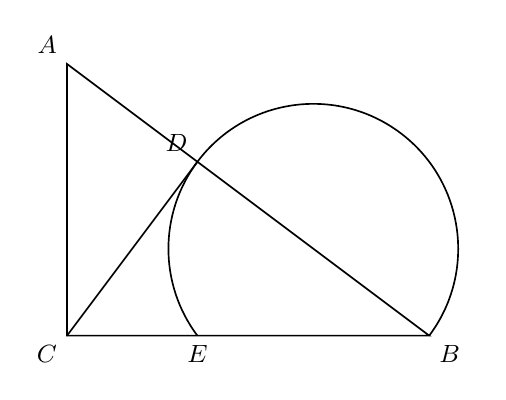
\begin{tikzpicture}[scale=1.15, semithick, font=\small]
  \coordinate (A) at (0,3);
  \coordinate (B) at (4,0);
  \coordinate (C) at (0,0);
  \coordinate (D) at (1.44,1.92);
  \coordinate (E) at (1.44,0);
  \draw (A) -- (C) -- (B) -- cycle;
  \draw (C) -- (D);
  \draw (4,0) arc[start angle=-36.87, end angle=216.87, radius=1.6];
  \node[above left] at (A) {$A$};
  \node[below left] at (C) {$C$};
  \node[below right] at (B) {$B$};
  \node[above left] at (D) {$D$};
  \node[below] at (E) {$E$};
\end{tikzpicture}
\end{center}
\nopagebreak[4]
（A）$CE\cdot CB=AD\cdot DB$；（B）$CE\cdot CB=AD\cdot AB$；（C）$AD\cdot AB=CD^2$；（D）$CE\cdot EB=CD^2$。

\end{question}
\begin{question}
\gkti{6}从 $0$，$2$ 中选一个数字，从 $1$，$3$，$5$ 中选两个数字，组成无重复数字的三位数，其中奇数的个数为\mbox{（　　）}

（A）$24$；（B）$18$；（C）$12$；（D）$6$。

\Needspace{0.4\textheight}
\end{question}
\begin{question}
\gkti{7}某三棱锥的三视图如图所示，该三棱锥的表面积是\mbox{（　　）}
\nopagebreak[4]
\begin{center}% 2012 年北京卷理科第 7 题：某三棱锥的三视图（正视图、侧视图、俯视图）。
% 来源 PDF：普通高考/2012/2012北京理.pdf，第 1 页（印面 719）中栏。
% 正视图：底 5（左段 2、右段 3），高 4；侧视图：底 4、高 4 的直角三角形；
% 俯视图：直角边 5 与 4 的直角三角形，顶点投影落在 5 的边上距左端 2 处，故有内部分割线。
\begin{tikzpicture}[scale=0.82, semithick,
  dim/.style={<->, >=Stealth, thin},
  lab/.style={font=\small}]
  % ---------- 正视图 ----------
  \begin{scope}
    \draw (0,0) -- (5,0) -- (2,4) -- cycle;
    \draw[dim] (0,-0.35) -- (2,-0.35);
    \node[below] at (1,-0.35) {2};
    \draw[dim] (2,-0.35) -- (5,-0.35);
    \node[below] at (3.5,-0.35) {3};
    \draw[dim] (-0.35,0) -- (-0.35,4);
    \node[left] at (-0.35,2) {4};
    \node[below] at (2.5,-1.0) {正（主）视图};
  \end{scope}
  % ---------- 侧视图 ----------
  \begin{scope}[shift={(7.0,0)}]
    \draw (0,0) -- (4,0) -- (0,4) -- cycle;
    \draw[dim] (0,-0.35) -- (4,-0.35);
    \node[below] at (2,-0.35) {4};
    \node[below] at (2,-1.0) {侧（左）视图};
  \end{scope}
  % ---------- 俯视图 ----------
  \begin{scope}[shift={(0.6,-6.2)}]
    \draw (0,4) -- (5,4) -- (5,0) -- cycle;
    \draw (2,4) -- (5,0);
    \node[below] at (2.5,-0.55) {俯视图};
  \end{scope}
\end{tikzpicture}
\end{center}
\nopagebreak[4]
（A）$28+6\sqrt5$；（B）$30+6\sqrt5$；（C）$56+12\sqrt5$；（D）$60+12\sqrt5$。

\Needspace{0.4\textheight}
\end{question}
\begin{question}
\gkti{8}某棵果树前 $n$ 年的总产量 $S_n$ 与 $n$ 之间的关系如图所示。从目前记录的结果看，前 $m$ 年的年平均产量最高，$m$ 的值为\mbox{（　　）}
\nopagebreak[4]
\begin{center}% 2012 年北京卷理科第 8 题：果树总产量 S_n 与年数 n 的散点图。
% 来源 PDF：普通高考/2012/2012北京理.pdf，第 1 页（印面 719）中栏。
% 图中共 9 个样本点 n=1,2,…,9；按原图逐点量取纵坐标（以横轴 1 个单位长为 1），
% 各点与原点连线的斜率依次为 0.05,0.05,0.29,0.47,0.63,0.65,0.86,0.88,0.89，故最大者在 n=9。
\begin{tikzpicture}[scale=0.70, semithick, >=Stealth]
  \draw[->] (0,0) -- (11.6,0) node[below] {$n$};
  \draw[->] (0,0) -- (0,8.6) node[left] {$S_n$};
  \node[below left] at (0,0) {$O$};
  \foreach \x in {1,...,11} {
    \draw (\x,0) -- (\x,-0.12);
    \node[below, font=\small] at (\x,-0.12) {\x};
  }
  \foreach \x/\y in {1/0.05, 2/0.05, 3/0.87, 4/1.88, 5/3.17, 6/3.89,
                     7/6.03, 8/7.03, 9/8.02} {
    \fill (\x,\y) circle (2.1pt);
  }
\end{tikzpicture}
\end{center}
\nopagebreak[4]
（A）$5$；（B）$7$；（C）$9$；（D）$11$。

\end{question}
\gkpart{二、填空题}

\begin{question}
\gkti{9}直线 $\begin{cases}x=2+t,\\y=-1-t,\end{cases}$（$t$ 为参数）与曲线 $\begin{cases}x=3\cos\alpha,\\y=3\sin\alpha,\end{cases}$（$\alpha$ 为参数）的交点个数为\gkblank{}。

\end{question}
\begin{question}
\gkti{10}已知 $\{a_n\}$ 为等差数列，$S_n$ 为其前 $n$ 项和，若 $a_1=\dfrac12$，$S_2=a_3$，则 $a_2=$\gkblank{}；$S_n=$\gkblank{}。

\end{question}
\begin{question}
\gkti{11}在 $\triangle ABC$ 中，若 $a=2$，$b+c=7$，$\cos B=-\dfrac14$，则 $b=$\gkblank{}。

\end{question}
\begin{question}
\gkti{12}在直角坐标系 $xOy$ 中，直线 $l$ 过抛物线 $y^2=4x$ 的焦点 $F$，且与该抛物线相交于 $A$，$B$ 两点，其中点 $A$ 在 $x$ 轴上方。若直线 $l$ 的倾斜角为 $60^\circ$，则 $\triangle OAF$ 的面积为\gkblank{}。

\end{question}
\begin{question}
\gkti{13}已知正方形 $ABCD$ 的边长为 $1$，点 $E$ 是 $AB$ 边上的动点，则 $\overrightarrow{DE}\cdot\overrightarrow{CB}$ 的值为\gkblank{}；$\overrightarrow{DE}\cdot\overrightarrow{DC}$ 的最大值为\gkblank{}。

\end{question}
\begin{question}
\gkti{14}已知 $f(x)=m(x-2m)(x+m+3)$，$g(x)=2^x-2$。若同时满足条件：① $\forall x\in\mathbf R$，$f(x)<0$ 或 $g(x)<0$；② $\exists x\in(-\infty,-4)$，$f(x)g(x)<0$，则 $m$ 的取值范围是\gkblank{}。

\end{question}
\gkpart{三、解答题}

\begin{question}
\gkti{15}已知函数 $f(x)=\dfrac{(\sin x-\cos x)\sin2x}{\sin x}$。

（1） 求 $f(x)$ 的定义域及最小正周期；

（2） 求 $f(x)$ 的单调递增区间。

\Needspace{0.4\textheight}
\end{question}
\begin{question}
\gkti{16}如图 1，在 $\mathrm{Rt}\triangle ABC$ 中，$\angle C=90^\circ$，$BC=3$，$AC=6$。$D$，$E$ 分别是 $AC$，$AB$ 上的点，且 $DE\parallel BC$，$DE=2$，将 $\triangle ADE$ 沿 $DE$ 折起到 $\triangle A_1DE$ 的位置，使 $A_1C\perp CD$，如图 2。

（1） 求证：$A_1C\perp$ 平面 $BCDE$；

（2） 若 $M$ 是 $A_1D$ 的中点，求 $CM$ 与平面 $A_1BE$ 所成角的大小；

（3） 线段 $BC$ 上是否存在点 $P$，使平面 $A_1DP$ 与平面 $A_1BE$ 垂直？说明理由。
\nopagebreak[4]
\begin{center}% 2012 年北京卷理科第 16 题：Rt△ABC（BC=3，AC=6）沿 DE（DE∥BC，DE=2）折起。
% 来源 PDF：普通高考/2012/2012北京理.pdf，第 1 页（印面 717）右栏。
% 图 1：D、E 分别在 AC、AB 上，DE=2；图 2：A 到 A1，A1C⊥CD，M 为 A1D 中点。
\begin{tikzpicture}[scale=0.78, semithick, font=\small]
  % ---------- 图 1 ----------
  \begin{scope}
    \coordinate (A) at (0,6);
    \coordinate (C) at (0,0);
    \coordinate (B) at (3,0);
    \coordinate (D) at (0,2);
    \coordinate (E) at (2,2);
    \draw (A) -- (C) -- (B) -- cycle;
    \draw (D) -- (E);
    \node[above left] at (A) {$A$};
    \node[below left] at (C) {$C$};
    \node[below right] at (B) {$B$};
    \node[left] at (D) {$D$};
    \node[above] at (E) {$E$};
    \node[below] at (1.5,-0.55) {图 1};
  \end{scope}
  % ---------- 图 2 ----------
  \begin{scope}[shift={(6.2,0)}]
    \coordinate (A1) at (0,4.9);
    \coordinate (C2) at (0.1,0.1);
    \coordinate (B2) at (3.8,0.1);
    \coordinate (D2) at (1.6,1.7);
    \coordinate (E2) at (3.3,2.0);
    \coordinate (M2) at (0.8,3.3);
    \draw (A1) -- (C2) -- (B2);
    \draw (A1) -- (D2);
    \draw (A1) -- (E2);
    \draw (A1) -- (B2);
    \draw (E2) -- (B2);
    \draw[dashed] (C2) -- (D2);
    \draw[dashed] (D2) -- (E2);
    \fill (M2) circle (1.6pt);
    \node[above left] at (A1) {$A_1$};
    \node[below left] at (C2) {$C$};
    \node[below right] at (B2) {$B$};
    \node[below left] at (D2) {$D$};
    \node[right] at (E2) {$E$};
    \node[left] at (M2) {$M$};
    \node[below] at (1.9,-0.55) {图 2};
  \end{scope}
\end{tikzpicture}
\end{center}
\nopagebreak[4]
\end{question}
\begin{question}
\gkti{17}近年来，某市为促进生活垃圾的分类处理，将生活垃圾分为厨余垃圾、可回收物和其他垃圾三类，并分别设置了相应的垃圾箱。为调查居民生活垃圾分类投放情况，现随机抽取了该市三类垃圾箱中总计 $1000$ 吨生活垃圾，数据统计如下（单位：吨）：

\begin{center}
\begin{tabular}{llll}
\toprule
垃圾类别 & “厨余垃圾”箱 & “可回收物”箱 & “其他垃圾”箱 \\
\midrule
厨余垃圾 & $400$ & $100$ & $100$ \\
可回收物 & $30$ & $240$ & $30$ \\
其他垃圾 & $20$ & $20$ & $60$ \\
\bottomrule
\end{tabular}
\end{center}

（1） 试估计厨余垃圾投放正确的概率；

（2） 试估计生活垃圾投放错误的概率；

（3） 假设厨余垃圾在“厨余垃圾”箱、“可回收物”箱、“其他垃圾”箱的投放量分别为 $a$，$b$，$c$，其中 $a>0$，$a+b+c=600$。当数据 $a$，$b$，$c$ 的方差 $s^2$ 最大时，写出 $a$，$b$，$c$ 的值（结论不要求证明），并求此时 $s^2$ 的值。

（注：$s^2=\dfrac1n\left[(x_1-\overline x)^2+(x_2-\overline x)^2+\cdots+(x_n-\overline x)^2\right]$，其中 $\overline x$ 为数据 $x_1$，$x_2$，$\cdots$，$x_n$ 的平均数）

\end{question}
\begin{question}
\gkti{18}已知函数 $f(x)=ax^2+1$（$a>0$），$g(x)=x^3+bx$。

（1） 若曲线 $y=f(x)$ 与曲线 $y=g(x)$ 在它们的交点 $(1,c)$ 处具有公共切线，求 $a$，$b$ 的值；

（2） 当 $a^2=4b$ 时，求函数 $f(x)+g(x)$ 的单调区间，并求其在区间 $(-\infty,-1]$ 上的最大值。

\end{question}
\begin{question}
\gkti{19}已知曲线 $C:(5-m)x^2+(m-2)y^2=8$（$m\in\mathbf R$）。

（1） 若曲线 $C$ 是焦点在 $x$ 轴上的椭圆，求 $m$ 的取值范围；

（2） 设 $m=4$，曲线 $C$ 与 $y$ 轴的交点为 $A$，$B$（点 $A$ 位于点 $B$ 的上方），直线 $y=kx+4$ 与曲线 $C$ 交于不同的两点 $M$，$N$，直线 $y=1$ 与直线 $BM$ 交于点 $G$。求证：$A$，$G$，$N$ 三点共线。

\end{question}
\begin{question}
\gkti{20}设 $A$ 是由 $m\times n$ 个实数组成的 $m$ 行 $n$ 列的数表，满足：每个数的绝对值不大于 $1$，且所有数的和为零。记 $S(m,n)$ 为所有这样的数表构成的集合。

对于 $A\in S(m,n)$，记 $r_i(A)$ 为 $A$ 的第 $i$ 行各数之和（$1\leqslant i\leqslant m$），$c_j(A)$ 为 $A$ 的第 $j$ 列各数之和（$1\leqslant j\leqslant n$）；记 $k(A)$ 为 $|r_1(A)|$，$|r_2(A)|$，$\cdots$，$|r_m(A)|$，$|c_1(A)|$，$|c_2(A)|$，$\cdots$，$|c_n(A)|$ 中的最小值。

\Needspace{5\baselineskip}
（1） 对如下数表 $A$，求 $k(A)$ 的值；

\nopagebreak[4]
\[\begin{array}{|c|c|c|}\hline 1 & 1 & -0.8\\ \hline 0.1 & -0.3 & -1\\ \hline\end{array}\]

\Needspace{5\baselineskip}
（2） 设数表 $A\in S(2,3)$ 形如

\nopagebreak[4]
\[\begin{array}{|c|c|c|}\hline 1 & 1 & c\\ \hline a & b & -1\\ \hline\end{array}\]

求 $k(A)$ 的最大值；

（3） 给定正整数 $t$，对于所有的 $A\in S(2,2t+1)$，求 $k(A)$ 的最大值。

\end{question}